\section{Related Work}
This section explores the related work inside the RTI area and explains the
underlying principles. The project is currently only concerned with the viewing
part, so that will covered in most depth.

\subsection{RTI Theory and Workflows}

The RTI workflow is a three step one (see~\autoref{capture}) in our context
(with the hunt for the physical object excluded). The object is placed central under
some capturing device (like~\autoref{dome}). A camera is
statically mounted on top. And the lights are setup to be lit in
order to have a different light position for all captured images. From these
images the RTI coefficents are calculated (see~\autoref{overview1}).

\fig{capture}{RTI Workflow}{RTI workflow, courtesy of CHI\cite*{noauthor_cultural_nodate-1}.}
\fig{dome}{RTI Dome}{RTI dome, from Malzbender et al.\cite*{malzbender_polynomial_2001}.}

\begin{figure}
\begin{subfloat}[]{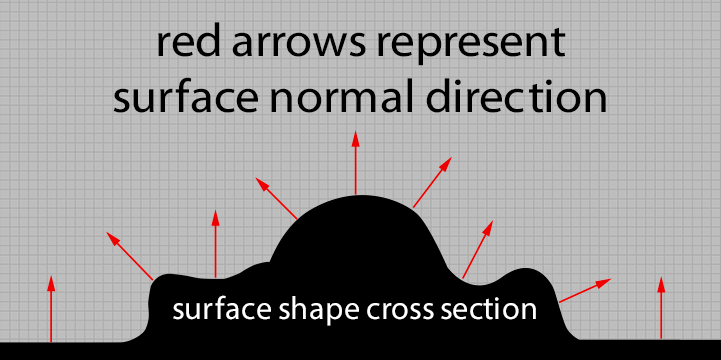
\includegraphics[max width=0.32\linewidth]{images/normals_01}}\end{subfloat}
\begin{subfloat}[]{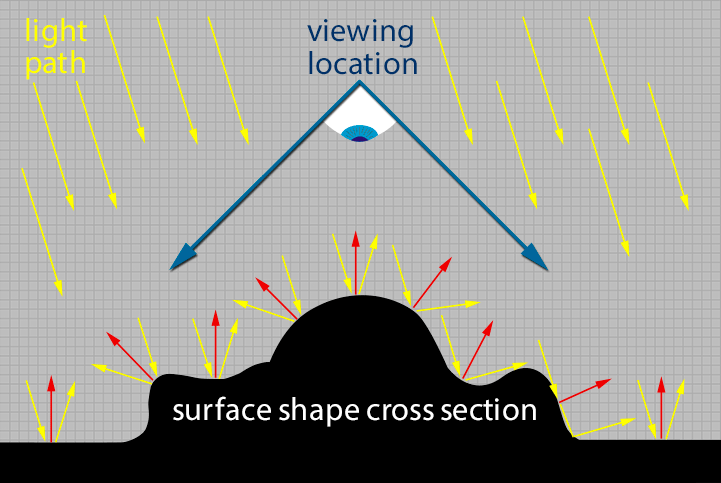
\includegraphics[max width=0.32\linewidth]{images/normals_02}}\end{subfloat}
\begin{subfloat}[]{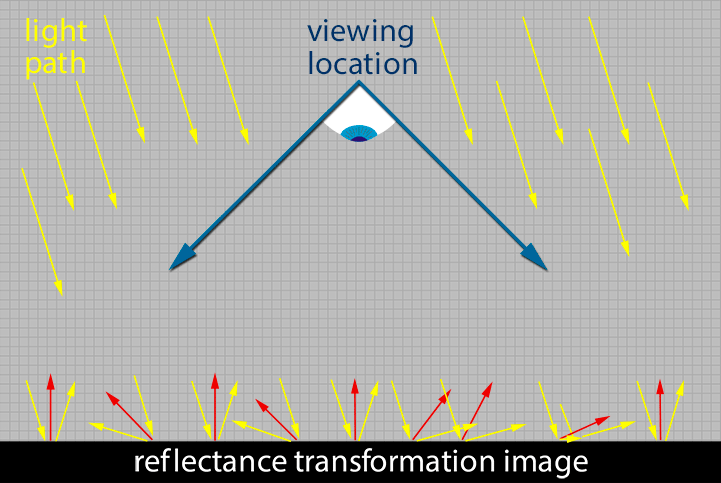
\includegraphics[max width=0.32\linewidth]{images/normals_03}}\end{subfloat}
\caption[RTI Overview]{(a) shows the to be captured object's normals.
  (b) shows the object with a single viewpoint and light source (in the
  capturing dome the eye would be camera). (c) visualizes the RTI viewing
  process. Images from CHI\cite*{noauthor_cultural_nodate}.}
\label{overview1}
\end{figure}

For example the PTM LRGB format\cite*{malzbender_polynomial_2001} stores 9
coefficients per texel: a0 - a5 for calculating the varying luminance and R, G, B
for colours, the resulting rendering is calculated in the following way per pixel:
\begin{align*}
R(u,v) = L(u,v)R_{n}(u,v);\\
G(u,v) = L(u,v)G_{n}(u,v);\\
B(u,v) = L(u,v)B_{n}(u,v);
\end{align*}
With u and v being the texture coordinates. $R_{n}$ ,$G_{n}$ and $B_{n}$ being
the raw unscaled input colours and $L(u, v)$ calculated as following:
\begin{equation*}
  L(u,v,l_{u},l_{v})=a_{0}(u,v)l_{u}^{2}+a_{1}(u,v)l_{v}^{2}+a_{2}(u,v)l_{u}l_{v}+a_{3}(u,v)l_{u}+a_{4}(u,v)l_{v}+a_{5}(u,v)
\end{equation*}
Where $a_{0}$-$a_{5}$ are the previously fit coefficients and $l_{u}$ and
$l_{v}$ are x and y components of the light vector projected into the texture
plane. The coefficients are calculated as part of the RTIBuilder process, for details refer to \cite*{malzbender_polynomial_2001}.
Other file formats will have slightly different sets of coefficients, but the
same principles hold, e.g. PTM RGB has 6 luminance coefficients per colour
channel and no fixed colours.

\subsection{Fileformats}\label{sec_relfile}
The most comprehensive overview on the current state of the art is done by the
American Library of Congress (LoC) as part of its digital preservation effort, with
sections on the ptm\cite{library_of_congress_polynomial_2018} and
rti\cite{library_of_congress_reflectance_2018} formats. The current PTM
specification by Malzbender et al\cite*{malzbender_polynomial_2001} from 2001 specifies 9
different formats, of which ``the most commonly used encoding formats are
[\ldots] PTM\_FORMAT\_LRGB (aka LRGB\ PTM) and
PTM\_FORMAT\_RGB (aka RGB PTM)''\cite{library_of_congress_polynomial_2018}, so most effort was
spent to support these inside the oxrti implementation. Both formats begin with
a metadata block consisting of 4 elements separated by newlines:
\begin{itemize}
\item The version prefix, which should be `PTM\_1.2' for recent files.
\item The format string, e.g. PTM\_FORMAT\_LRGB.
\item Image size, the dimensions in pixels.
\item Scales and biases, to scale and bias the coefficients before calculation.
\end{itemize}
This metadata block is followed by the raw texel data in forms depending on the
format All in reversed scanline order. PTM\_FORMAT\_RGB stores $a_{0}$-$a_{5}$ per
texel in separated RGB blocks. PTM\_FORMAT\_LRGB stores $a_{0}$-$a_{5}$ per texel
first, then followed by RGB blocks of a single coefficient per texel. The
destructuring of these is presented in detail in~\autoref{sec_ptmconverter}. Different
embedded JPEG compression styles are specified as well, but due to their
relatively small popularity and increased complexity skipped over for the inital
oxrti version.

The \.RTI fileformat specification by Corsini et al.\cite*{corsini_rti_2010} is a
newer format supporting Hemi-Spherical Harmonics (HSH) in addition to PTM's
biquadratic polynomials, as HSH ``handles shiny surfaces and specular
highlights (bright spots of light appearing on shiny objects) better than PTM,
which yields matte images.''\cite*{library_of_congress_reflectance_2018}. One
additional difference is the support of metadata as an XMP packet at the end of
the file. As most locally available data is in PTM format, support for the RTI
format is initially skipped for this project, but it will be easy to add support
in the future.

\subsection{RTI Viewers}
Following RTI Viewers are currently available:
\begin{description}
\item[PTM Viewer]  from HP. The inital viewer application, available at
  \cite*{noauthor_hp_nodate}. Downloads for Windows, MacOS, HP-UX and Linux.
  Only rudimentary functionality of changing the light direction. The MacOS
  version did not run on the author's computer. No source code available.
\item[RTIViewer] available from the CHI at \cite*{noauthor_cultural_nodate-1}.
  Most widely used viewer. Downloads for Windows and MacOS\@. Source code only available per request:
  ``This software is available under the Gnu General Public License version 3.
  If you wish to receive a copy of the source code, please send email to
  info@c-h-i.org.'' PTM and RTI formats supported. Features: Light control, multiple rendering
  modes, bookmarks.
\item[InscriptiFact Viewer] by the University of Southern California. Offered in two flavours, a downloadable Java
  program\cite*{noauthor_inscriptifact_nodate-1} and a embedded Java
  applet\cite*{noauthor_inscriptifact_nodate} (not working as of \today). No
  source code available. Features: Light control, multiple rendering modes.
\item[webRTIViewer] by the Visual Computing Laboratory. Download at
  \cite*{noauthor_reflectance_nodate}. Support for a proprietary format,
  requiring pre-processing with a C++ command line utility. Source code
  included in the download. Features: Light control.
\item[OxRTI SVG Viewer] by Christopher Ramsey. SVG based web viewer available at
  \cite*{noauthor_oxrti_nodate}, developed at the same time as this project.
  Requiring pre-processed PTMs. No source code available. Features: Light control, multiple rendering modes,
  comments and painting.
\end{description}
